\chapter{Project Planning and Design}

\section{UML Diagrams}

UML, or Unified Modeling Language, is a standardized modeling language that consists of a set of diagrams used for modeling business processes and documenting software systems, helping better communicating potential designs and architectural decisions \parencite{uml}. 

The most common UML diagrams include:
\begin{itemize}
    \item \textbf{Use Case Diagram} - Illustrates the system's intended functionality in terms of actors, use cases, and their relationships, showing how the system delivers value to users.
    \item \textbf{Class Diagram} - Depicts the structure of the system by showing classes, attributes, operations, and static relationships between classes.
    \item \textbf{Sequence Diagram} - Demonstrates how objects interact in a particular, timed sequence scenario, focusing on the messages passed between objects.
    \item \textbf{Activity Diagram} - Represents the workflow of a target use case or business process through a series of activities, emphasizing steps, choices, iterations, and concurrency.
\end{itemize}

The student has used UML diagrams to present the stakeholders with a visual representation of the system's design and architecture. The diagrams can be found below.

\subsection{Use Case Diagram}

\begin{figure}[ht]
    \centering
    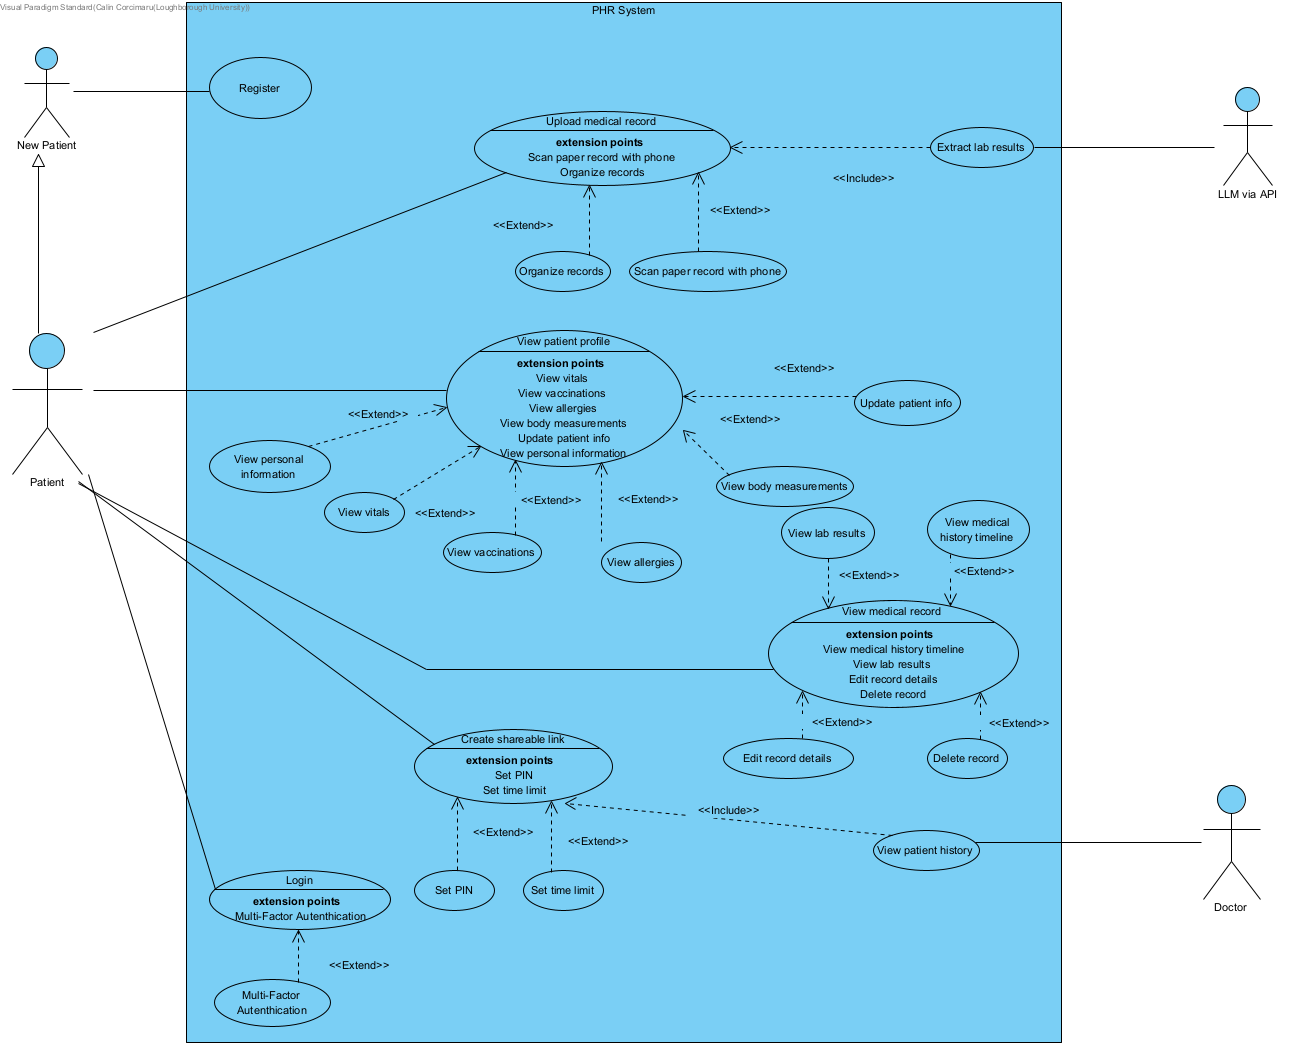
\includegraphics[width=\textwidth,height=0.8\textheight,keepaspectratio]{Use_Case.png}
    \caption{UML Use Case Diagram}
    \label{fig:uml_usecase}
\end{figure}

\FloatBarrier
\clearpage

\subsection{Use Case Specifications}

\subsubsection{Login}
\begin{tabular}{|p{0.2\textwidth}|p{0.7\textwidth}|}
\hline
Description & The Login use case allows the app user to log in to their existing account via their credentials, with an optional use of MFA. \\
\hline
Actors & Patient \\
\hline
Preconditions & Must have an existing account \\
\hline
Steps & 1. User enters user and password \newline
       2. User clicks on the login button \newline
       3. App validates user credentials \newline
       4. Patient enters MFA code if enabled \newline
       5. App logs user in \\
\hline
\end{tabular}

\subsubsection{Register}
\begin{tabular}{|p{0.2\textwidth}|p{0.7\textwidth}|}
\hline
Description & The Register use case allows the app user to create a new account. \\
\hline
Actors & New Patient \\
\hline
Preconditions & No existing account with the email used to register \\
\hline
Steps & 1. User enters user and password \newline
       2. User clicks on the register button \newline
       3. App validates user credentials \newline
       4. App logs user in \newline
       5. App sends verification email \newline
       6. User verifies email \\
\hline
\end{tabular}

\subsubsection{Upload Record}
\begin{tabular}{|p{0.2\textwidth}|p{0.7\textwidth}|}
\hline
Description & The Upload Record use case allows the patient to upload their medical records to the app. \\
\hline
Actors & Patient, LLM \\
\hline
Preconditions & Must be logged in \\
\hline
Steps & 1. User selects file upload (or camera scan) \newline
       2. User selects the record to upload \newline
       3. User clicks on the upload button \newline
       4. App validates the record \newline
       5. User selects the appropriate record type \newline
       6. If record type is lab result, app sends the record to LLM via API for processing into JSON format \newline
       7. App adds the record to the database \newline
       8. App shows confirmation to user \\
\hline
\end{tabular}

\subsubsection{Share Records}
\begin{tabular}{|p{0.2\textwidth}|p{0.7\textwidth}|}
\hline
Description & The Share Records use case allows the patient to share their medical records with doctors. \\
\hline
Actors & Patient, Doctor \\
\hline
Preconditions & Must be logged in and have records uploaded \\
\hline
Steps & 1. User selects option to create a share link \newline
       2. OPTIONAL: User selects the records to share \newline
       3. OPTIONAL: User adds a PIN to the share link \newline
       4. User selects time limit for the share link \newline
       5. App generates the share link \newline
       6. App sends the share link to the doctor via email \newline
       7. App shows confirmation to user \newline
       8. Doctor clicks on the share link \newline
       9. Doctor enters the PIN (if required) \newline
       10. App validates the PIN \newline
       11. App shows the records to the doctor \\
\hline
\end{tabular}

\subsubsection{View Records}
\begin{tabular}{|p{0.2\textwidth}|p{0.7\textwidth}|}
\hline
Description & The View Records use case allows the patient to view and edit their uploaded medical records. \\
\hline
Actors & Patient \\
\hline
Preconditions & Must be logged in and have records uploaded \\
\hline
Steps & 1. App provides a list of records or medical history \newline
       2. User selects record to view from list or medical history \newline
       3. App retrieves the record from the database \newline
       4. App shows the record to the user \newline
       5. OPTIONAL: User can view the record in a graphical format if lab result \newline
       6. OPTIONAL: User edits the record \newline
       7. OPTIONAL: User deletes the record \\
\hline
\end{tabular}

\subsubsection{View Patient Profile}
\begin{tabular}{|p{0.2\textwidth}|p{0.7\textwidth}|}
\hline
Description & The View Patient Profile use case allows the patient to view and edit their profile information, including health information such as allergies, medications, vaccinations and recorded health data like blood pressure, glucose levels, etc. \\
\hline
Actors & Patient \\
\hline
Preconditions & Must be logged in \\
\hline
Steps & 1. User selects the profile section \newline
       2. App retrieves the profile information from the database \newline
       3. App shows the profile information to the user - vaccinations, allergies, medications, health data \newline
       4. OPTIONAL: User edits the profile information \newline
       5. OPTIONAL: User adds new health data \newline
       6. OPTIONAL: User deletes health data \newline
       7. OPTIONAL: User can view health data in a graphical format \\
\hline
\end{tabular}

\FloatBarrier
\clearpage

\subsection{Class Diagram}
\begin{figure}[htbp]
    \centering
    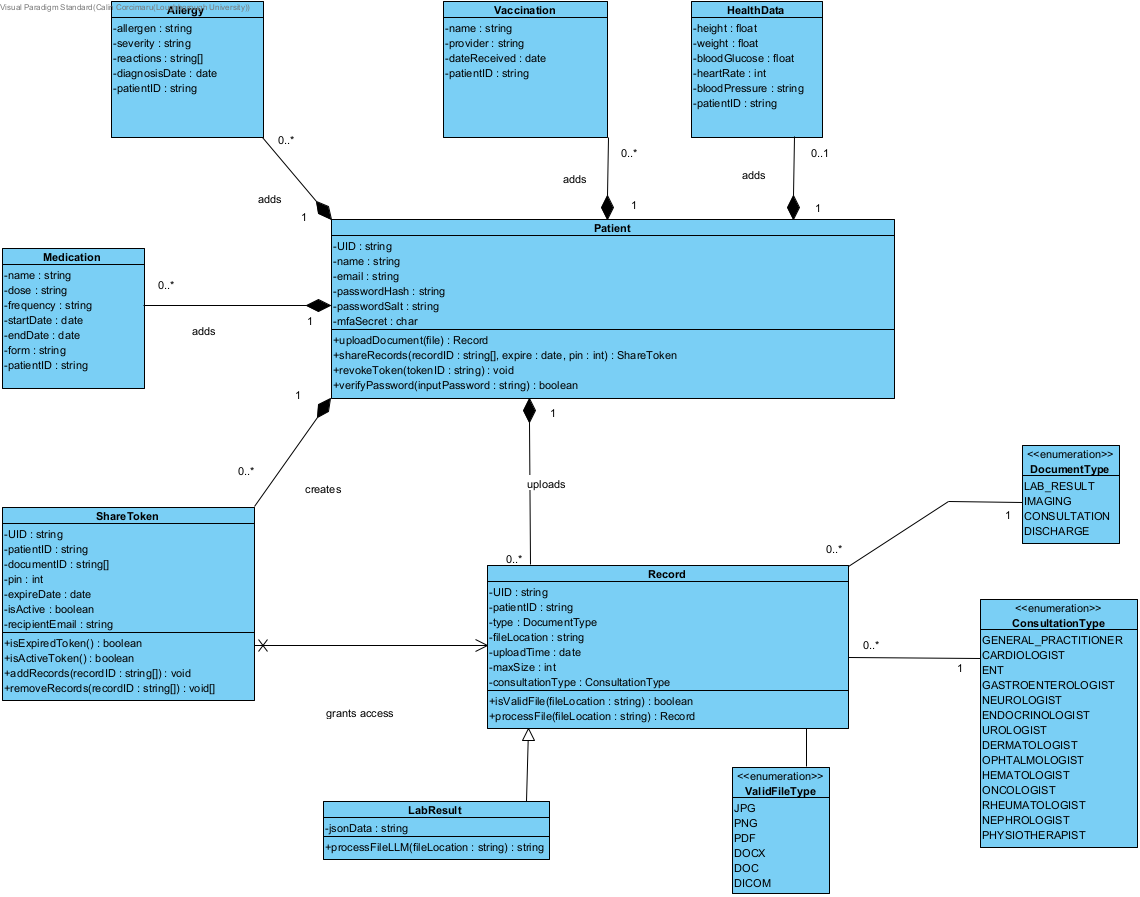
\includegraphics[width=\textwidth,height=0.8\textheight,keepaspectratio]{Class_diagram.png}
    \caption{UML Class Diagram}
    \label{fig:uml_class}
\end{figure}

\FloatBarrier
\clearpage

\subsection{Sequence Diagrams}
\begin{figure}[htbp]
    \centering
    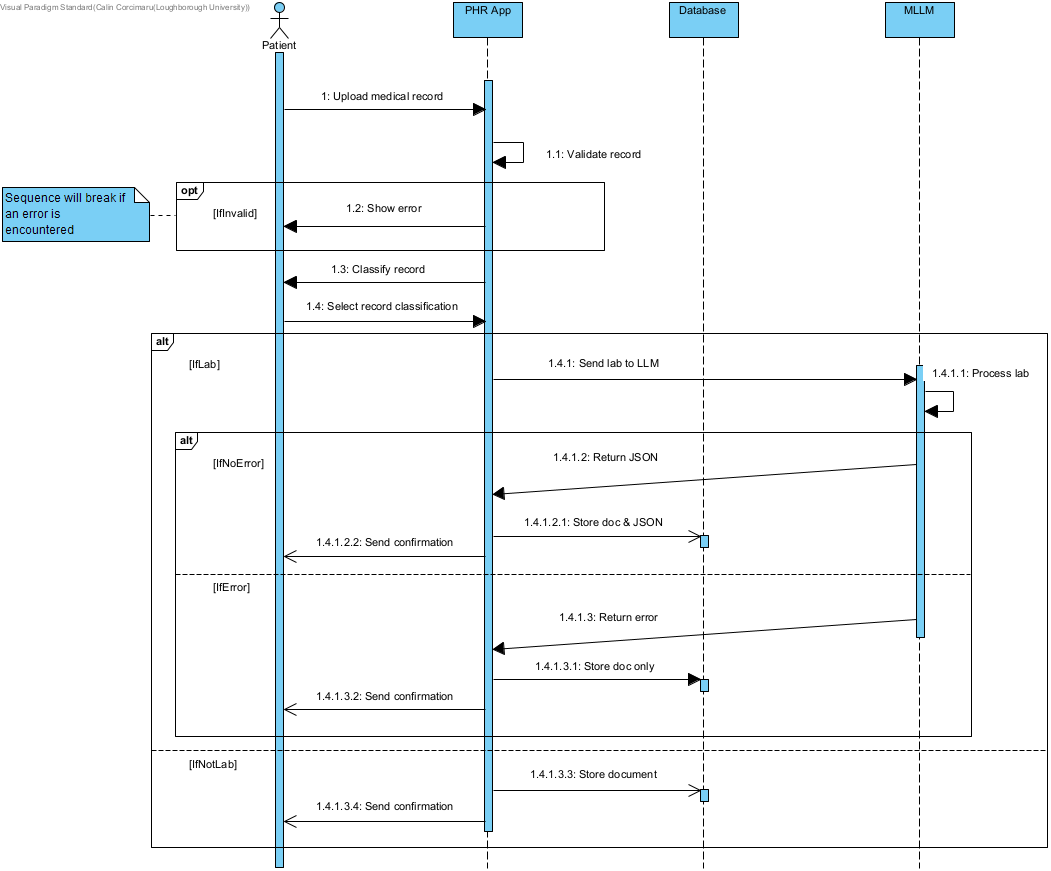
\includegraphics[width=\textwidth,height=0.8\textheight,keepaspectratio]{Sequence_upload.png}
    \caption{UML Sequence Diagram - Upload Record Use Case}
    \label{fig:sequence1}
\end{figure}

\begin{figure}[htbp]
    \centering
    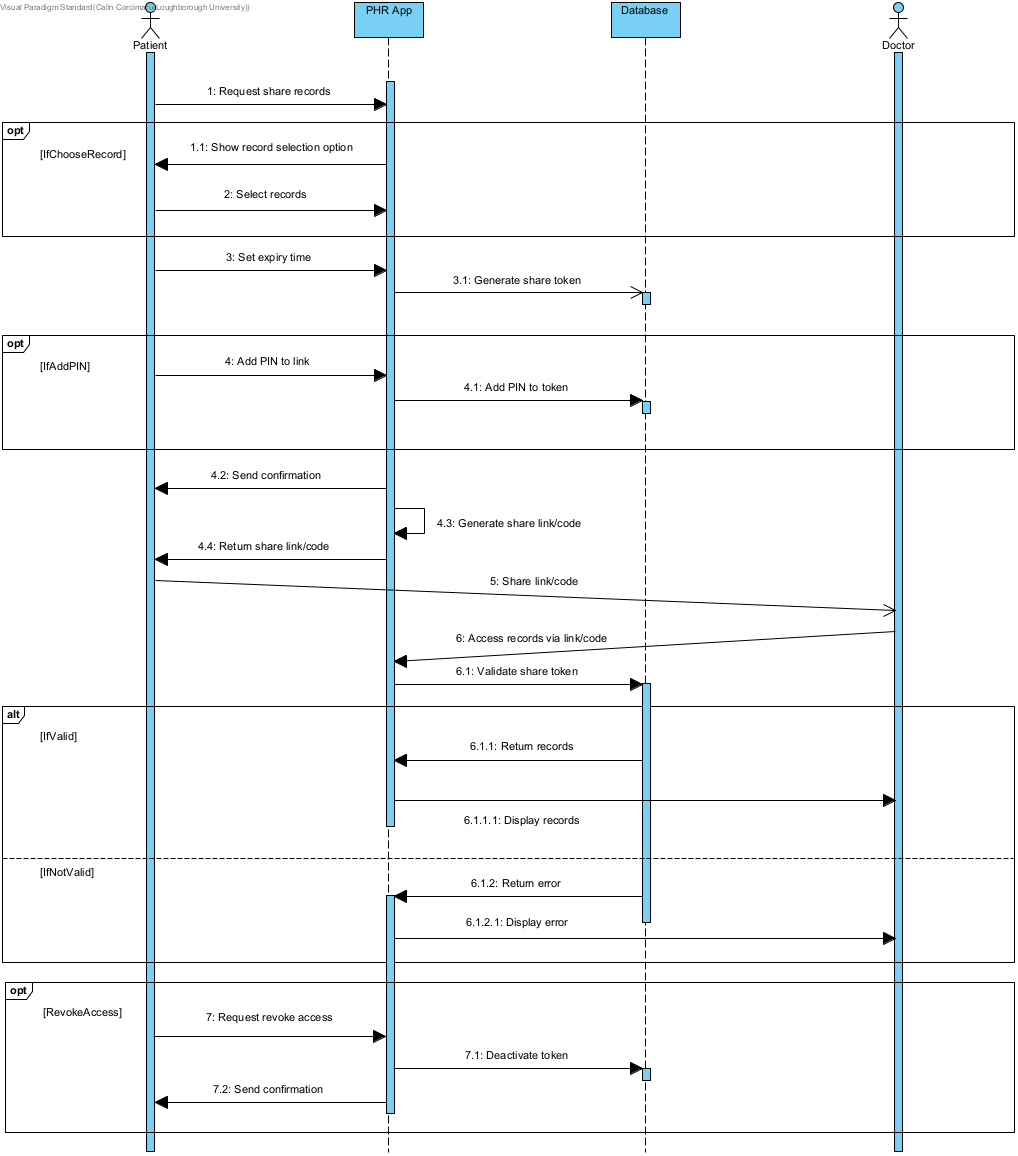
\includegraphics[width=\textwidth,height=0.8\textheight,keepaspectratio]{Sequence_share.png}
    \caption{UML Sequence Diagram - Share Records Use Case}
    \label{fig:sequence2}
\end{figure}

\FloatBarrier

\noindent\begin{minipage}{\textwidth}
    \subsection{Activity Diagrams}
    \begin{center}
        \rotatebox[origin=c]{270}{
            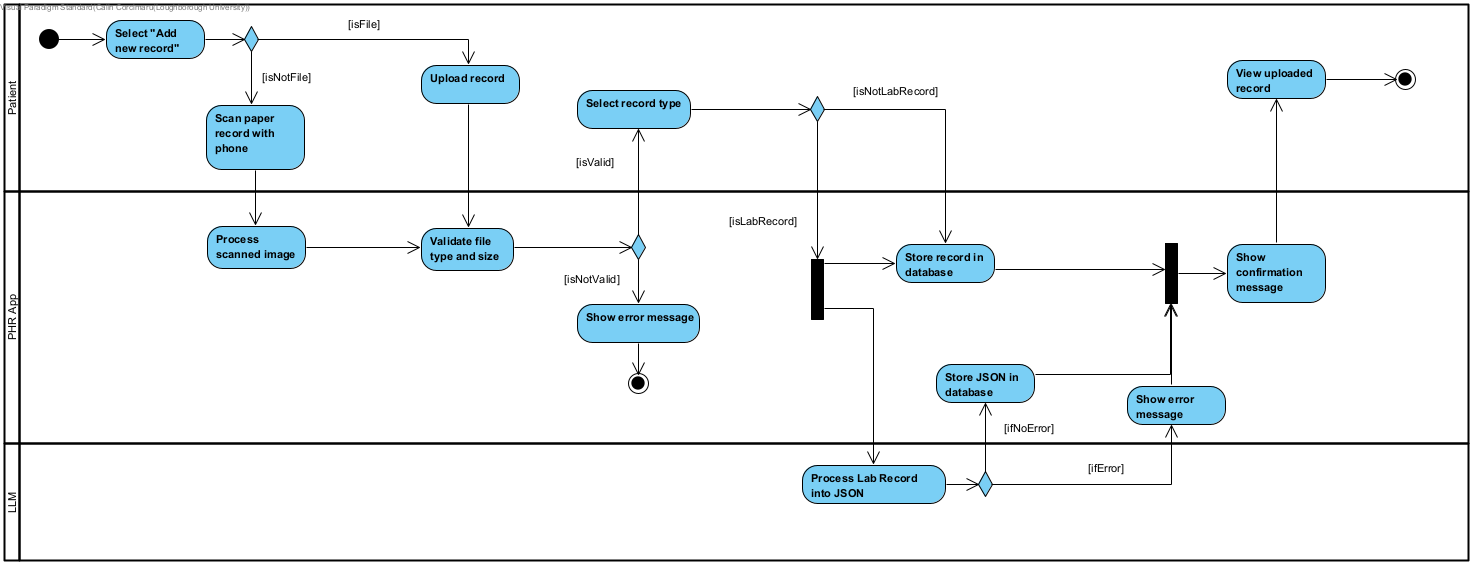
\includegraphics[width=0.9\textheight,keepaspectratio]{Activity_upload.png}
        }
        \captionof{figure}{UML Activity Diagram - Upload Record Use Case}
        \label{fig:activity1}
    \end{center}
\end{minipage}

\noindent\begin{minipage}{\textwidth}
    \begin{center}
        \rotatebox[origin=c]{270}{
            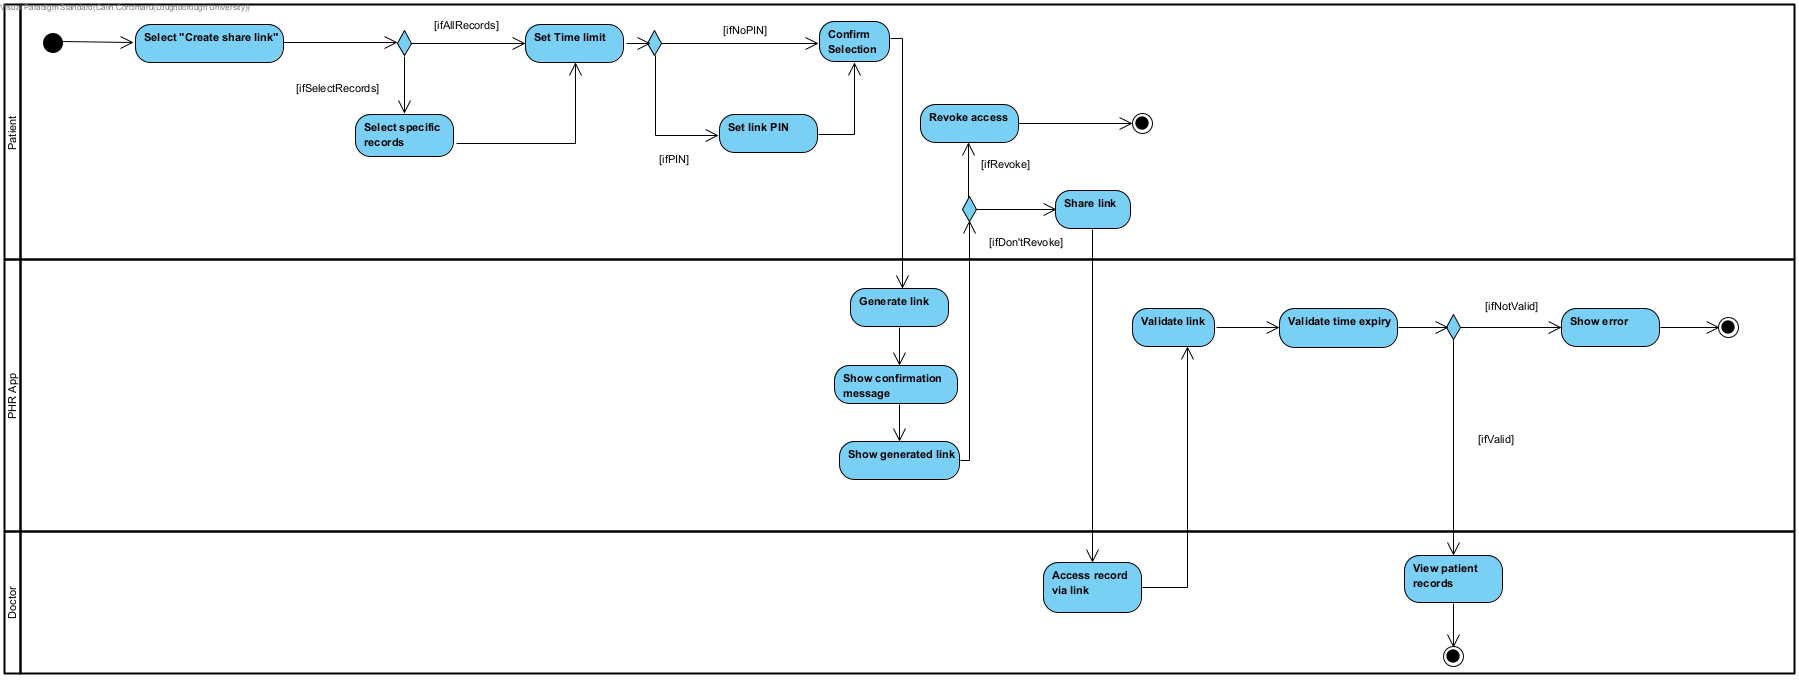
\includegraphics[width=0.9\textheight,keepaspectratio]{Activity_link.png}
        }
        \captionof{figure}{UML Activity Diagram - Share Records Use Case}
        \label{fig:activity2}
    \end{center}
\end{minipage}

\FloatBarrier

\noindent\begin{minipage}{\textwidth}
    \section{Database Design}
    \begin{center}
        \rotatebox[origin=c]{270}{
            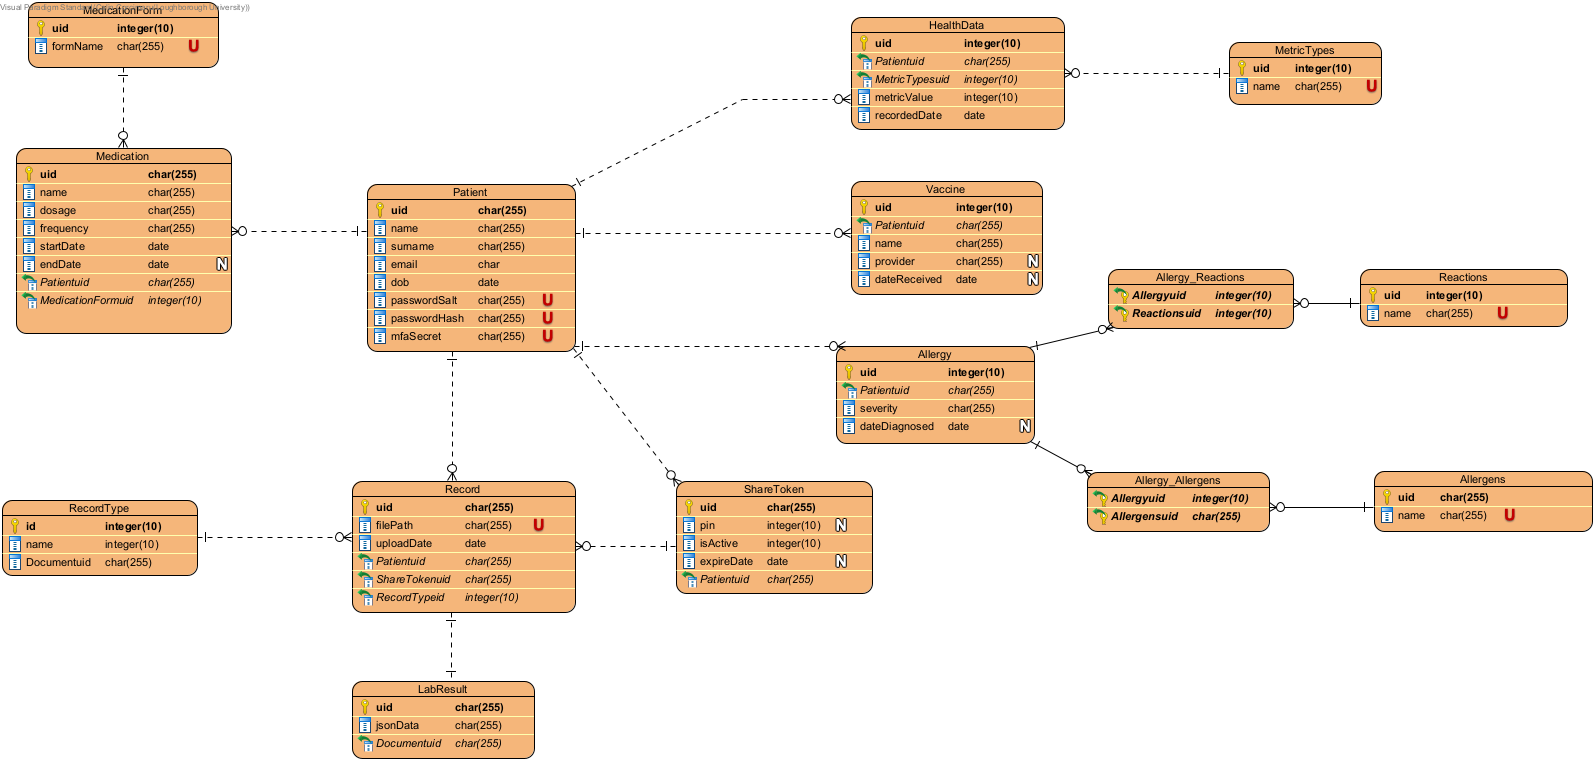
\includegraphics[width=0.9\textheight,keepaspectratio]{ERD.png}
        }
        \captionof{figure}{Entity Relationship Diagram}
        \label{fig:erd}
    \end{center}
\end{minipage}

\FloatBarrier

\section{Wireframes}

\section{Project Tech Stack}

\subsection{Frontend}

\subsection{Backend}

\subsection{Database}

\section{Project Management}

\subsection{Methodology and Tools}

Based on the research above, the student has decided that he will be using a hybrid approach, with Waterfall as the main methodology for planning managing the project. The development part of the project will be done using ScrumBan, so that the student will be able to utilise elements from both frameworks. There are several reasons for this choice:

\begin{enumerate}
    \item The nature of the project - the student is working on a project that has a limited timeframe (about 6-7 months) and is of a smaller scale. 
    \item Documentation requirements - the student is required to document the progress during the project in this report, including the requirements gathered, design considerations and implementation decisions and outcomes. 
    \item Regulatory requirements - the student is required to adhere to the regulations and standards of the healthcare industry, which may require extensive documentation and planning.
    \item Customer involvement - the student will be working closely with the project stakeholder, who will be providing feedback and guidance throughout the project.
    \item Familiarity with both Agile and Waterfall - the student has experience with both Agile (specifically Scrum and Kanban) and Waterfall methodologies, and has worked on projects that have used both approaches.
\end{enumerate}

The student will use Jira Software as their project management tool, which is one of the most popular project management tool for software development projects that supports working with Agile frameworks such as Scrum and Kanban \parencite{atlassian}. The student has experience with Jira Software, having used it in previous projects, and is familiar with its features and capabilities.

\subsection{Project Backlogs}

\subsection{Sprints planning}